%---------Definicion de paquetes base--------------
\documentclass[12pt,letterpaper]{article}
\usepackage[utf8]{inputenc}
\usepackage{amsmath}
\usepackage{amsfonts}
\usepackage{amssymb}
\usepackage{url}
\usepackage{graphicx} 
\usepackage{float}
\usepackage{setspace}   %Allows double spacing with the \doublespacing command
\usepackage{fancyvrb} % verbatim replacement that allows latex
\usepackage{enumitem}
\usepackage{tabularx}
\usepackage{booktabs} % Required for nicer horizontal rules in tables
\usepackage[spanish, es-tabla, es-nodecimaldot]{babel}		%Separacion silabica espanola
\usepackage[left=2.00cm, right=2.00cm, top=2.00cm, bottom=2.00cm]{geometry}
\usepackage{multicol}	% Para manejar columnas multiples
\usepackage{longtable}  % Para manejar tablas de varias paginas con encabezado
		\newenvironment{Table}
		{\par\medskip\noindent\minipage{\linewidth}}
		{\endminipage\par\medskip}
\usepackage{fancyhdr}	% Para manejar los encabezados y pies de pagina
		\pagestyle{fancy}		% Contenido de los encabezados y pies de pagina
\usepackage{wrapfig}	% Necesario para la rubrica de evaluacion
\usepackage{helvet}
\renewcommand{\familydefault}{\sfdefault}
\graphicspath{{/home/noxd/Documents/documentos/}{/home/noxd/Doc/Temas selectos/Mauricio/gwr/}} %Setting the graphicspath
%--------Encabezado y pie de página---------------------
\lhead{Geoinformática}
\chead{}
\rhead{GWR}	% va el numero de experimento, al igual que en el titulo
\lfoot{PCIG}
\cfoot{\thepage\ }
\rfoot{CentroGeo}
%-----------Portada---------------------------------------------
\author{
Jorge Eduardo Cárdenas A.\\
Leonardo Coronado Arvayo\\
Jeziret Sahadi González Gallardo\\
{\small }\\
\vspace*{2.25in}}
\title{	
\includegraphics[width=8cm]{Logo} \\
\vspace*{.25in}
Tarea: \\ Regresión ponderada geográficamente \\
(GWR) \\
\vspace*{1.0in}}
%-----------Reporte----------------------------
\linespread{1.5}%
%	Portada y tabla de contenidos
\begin{document}
	\pagenumbering{gobble} % Remove page numbers (and reset to 1)
	\maketitle
\newpage
	\pagenumbering{arabic}
	\tableofcontents
\pagebreak





%====================================================================================================
%============================================introducción==============================================
%====================================================================================================
\section{Introducción}

En la presente tarea se repasa la regresión geográficamente ponderada (GWR, por sus siglas en ingles), para observar relaciones de características de poblaciones vulnerables con el índice de marginación a nivel municipio de México en 2015.

Para poder aplicar el GWR la librería MGWR de Python, primero se transforman los datos municipales al centroide del mismo (ya que se requieren las coordenadas de los datos y la base no los traía originalmente) y se obtienen las coordenadas usando QGIS. Seguido se normalizan los datos, se busca el valor de banda que minimiza el error de la regresión (usando el criterio de información Akaike y se aplica la GWR y se muestran los resultados de la regresión.

Por último, debido a que esta regresión se realiza localmente, es posible estimar indicadores en cada ubicación y mapearlos, en este caso, se grafican los valores de la bondad de ajuste $R^2$ para cada municipio de México.

%====================================================================================================
%============================================Metodologia==============================================
%====================================================================================================
\section{Metodología}

Esta sección se separa en una subsección de los cambios que se le realizaron a los datos para poder aplicar la GWR y en otra que explica brevemente como funciona esta regresión.

\subsection{Datos}

Los datos para esta práctica se obtuvieron en CONAPO \cite{a}, en este caso es la Cartografía de marginación por municipio 2015, que se puede ver en la Figura 1.

Debido a que la GWR funciona con puntos, ya que pondera la distancia de un dato a otro, se redujeron los municipios a los centroides de los mismos, lo cual fue principalmente necesario debido a que los datos no tenían coordenadas y se requerían los centroides para asignar coordenadas a los “puntos” o valores de cada municipio, ambos procedimientos se realizaron usando las herramientas de vectores de QGIS. 

\begin{figure}[H]
	\centering
	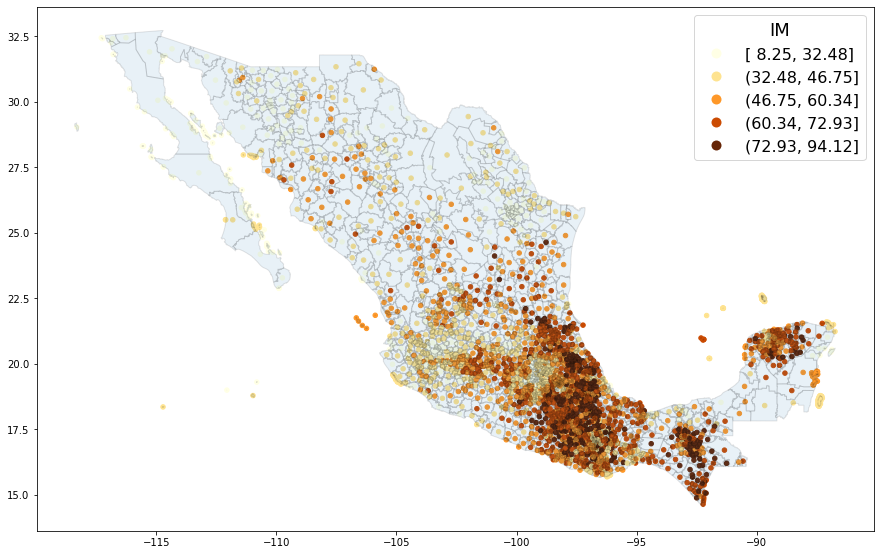
\includegraphics[scale=0.5]{output_6_1.png}
	\caption{IMM 2015 y sus centroides por IM 2015 con intervalos Fisher-Jenks}
\end{figure}

\subsection{GWR}

GWR es una técnica no estacionaria que modela relaciones espaciales geográficamente, de forma que los coeficientes $\beta$ dependen de la ubicación espacial, esta regresión tiene la forma \cite{b}: 

\begin{equation*}
	y_i = \beta_{i0} + \sum_{k=1}^{m} \beta_{ik} x_{ik} + e_i
\end{equation*}

Donde $y_i$ es la variable dependiente en la ubicación i, $x_{ik}$ son el set de variables independientes o explicativas, $\beta_{ik}$ son las constantes de regresión (de la k-ésima variable en la ubicación i), $\beta_{i0}$ es el intercepto en la ubicación i y $e_i$ es el error del modelo. 

El método se resuelve usando mínimos cuadrados con la inclusión de una matriz de pesos W que es la agrupación o acumulación de los pesos ponderados por la distancia \cite{b}. La ponderación de distancias, en la forma gaussiana, en su forma matricial es:


\begin{equation*}
W = 
\begin{pmatrix}
exp[-(\frac{b}{d_{1,1}})^2] & 0 & \cdots & 0 \\
0 & exp[-(\frac{b}{d_{2,2}})^2] & \cdots & 0 \\
\vdots  & \vdots  & \ddots & \vdots  \\
0 & 0 & \cdots & exp[-(\frac{b}{d_{t,t}})^2]
\end{pmatrix}
\end{equation*}

Donde b es una constante y $d_ij$ es la distancia euclidiana para un elipsoide y debe tener una forma similar a \cite{d}:

\begin{equation*}
d_{i,i} = \sum_{j=1}^{T} \sqrt{ (k_{1} (lat_i-lat_j)  )^2 
	+ (k_{2} (lon_i-lon_j) )^2  }
\end{equation*}

$lat_i$ es la latitud en i, $lon_i$ es la longitud en i,  $K_1$ y $K_2$ son variables que dependen de la variación de latitud.


El módulo de Python, MGWR, requiere que la variable dependiente se reajuste a valores de -1 a 1 para facilitar el algoritmo de ponderación de distancias que busca encontrar el valor de b que minimiza el error o criterio de información de Akaike de la GWR, de acuerdo a lo que se le indique.

%====================================================================================================
%============================================Resultados==============================================
%====================================================================================================
\section{Resultados}

En este caso, la regresión planteada es el índice de marginación (IM), contra la población que vive en localidades con menos de 5 mil personas (P5m), el porcentaje de la población que gana menos de 2 salarios mínimos (P2s) y la proporción de la población sin educación primaria (PSP). De forma que la ecuación es: 

\begin{equation*}
	IM_i=  \beta_{i0} +\sum_{k=1}^{m} \beta_{ik} P5m_{ik} +\sum_{j=1}^{m} \beta_{ij} P2s_{ij} +\sum_{q=1}^{m} \beta_{iq} PSP_{iq}+ e_i
\end{equation*}

Los resultados para un tipo de ponderación gaussiana se presentan en el siguiente cuadro de código, se observa primero los resultados de la regresión global y después para la regresión geográfica ponderada. En el caso de la regresión global tiene una bondad de ajuste global $R^2$ relativamente baja (0.479), sin embargo, todas las variables son significativas al 1\% para explicar al IM con excepción del intercepto. 

Todas las variables explicativas tienen una relación positiva con el IM, es decir que lo aumentan, así mismo, en magnitud la proporción de la población sin estudios de primaria y la que gana menos de dos salarios mínimos tienen un mayor efecto en IM que las localidades pequeñas (con menos de 5 mil habitantes).


\begin{figure}[H]
\begin{Verbatim}[baselinestretch=1]
===========================================================================
Model type                                                         Gaussian
Number of observations:                                                2857
Number of covariates:                                                     4

Global Regression Results
---------------------------------------------------------------------------
Residual sum of squares:                                           1487.263
Log-likelihood:                                                   -3121.333
AIC:                                                               6250.666
AICc:                                                              6252.687
BIC:                                                             -21215.563
R2:                                                                   0.479
Adj. R2:                                                              0.479

Variable                              Est.         SE  t(Est/SE)    p-value
------------------------------- ---------- ---------- ---------- ----------
cte                                  0.000      0.014      0.000      1.000
P5m                                  0.070      0.018      3.915      0.000
P2s                                  0.289      0.016     18.217      0.000
PSP                                  0.448      0.019     23.549      0.000
===========================================================================
\end{Verbatim}
\caption{Resumen de resultados de la regresión global}
\end{figure}

En comparación, la GWR tiene menor suma de errores al cuadrado, así como menor criterio de información Akaike, ambos indicando que esta regresión presenta un mejor ajuste. La bondad de ajuste aumenta a casi 80 \% y existe un valor del intercepto (en la anterior era aparentemente 0).

A su vez, el valor de los coeficientes cambia, tomando mayor relevancia en magnitud el coeficiente de la población que vive en localidades con menos de 5 mil personas y relativamente menos el peso la población que gana menos de 2 salarios mínimos. También en la proporción de la población sin educación primaria aumenta la magnitud del coeficiente. Todos los coeficientes caen dentro del intervalo de confianza. 

\begin{figure}[H]
\begin{Verbatim}[baselinestretch=1]
Geographically Weighted Regression (GWR) Results
---------------------------------------------------------------------------
Spatial kernel:                                           Adaptive bisquare
Bandwidth used:                                                      81.000

Diagnostic information
---------------------------------------------------------------------------
Residual sum of squares:                                            575.377
Effective number of parameters (trace(S)):                          309.244
Degree of freedom (n - trace(S)):                                  2547.756
Sigma estimate:                                                       0.475
Log-likelihood:                                                   -1764.732
AIC:                                                               4149.952
AICc:                                                              4225.813
BIC:                                                               5998.239
R2:                                                                   0.799
Adjusted R2:                                                          0.774
Adj. alpha (95\%):                                                    0.001
Adj. critical t value (95\%):                                         3.415

Summary Statistics For GWR Parameter Estimates
---------------------------------------------------------------------------
Variable                   Mean        STD        Min     Median        Max
-------------------- ---------- ---------- ---------- ---------- ----------
cte                       0.290      0.560     -1.289      0.322      2.478
P5m                       0.225      0.548     -2.086      0.097      3.114
PS2                       0.183      0.219     -0.832      0.176      1.033
PSP                       0.590      0.593     -0.721      0.382      2.940
===========================================================================
\end{Verbatim}
\caption{Resumen de resultados de la regresión geográficamente ponderada}
\end{figure}

\subsection{Bondad de ajuste $R^2$ local}

Como la GWR es calculada independientemente para cada observación, es posible calcular parámetros para cada ubicación \cite{c}. Estos valores se pueden encontrar y graficar o mapear, de forma que se puede visualizar la “magnitud” estadística de la relación entre las variables independientes y la dependiente \cite{c}. A continuación, se realiza esto para diferentes tipos de separaciones de intervalos. 

En las figuras 4, 5 y 6 se observa que hay valores muy altos de $R^2$ locales en el centro y noroeste del país y valores bajos alrededor del centro y al sureste. Cabe denotar que la zona que rodea a la Ciudad de México está rodeada por valores muy altos de $R^2$ que se puede interpretar con lugares donde el índice de marginación es causado muy fuertemente por localidades con menos de 5 mil habitantes, por altas proporciones de la población que gana menos de dos salarios mínimos y/o que no tiene educación primaria en esas ubicaciones. 



\begin{figure}[H]
	\centering
	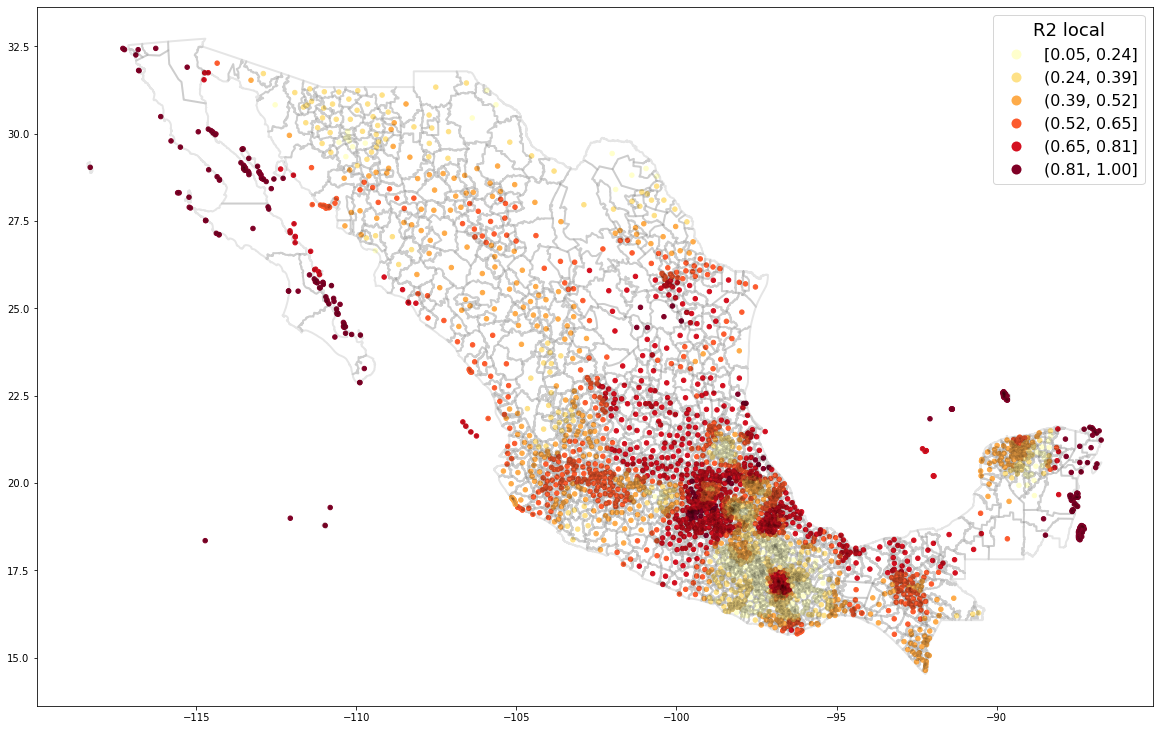
\includegraphics[scale=0.4]{output_17_1.png}
	\caption{Bondad de ajuste local usando separación Fisher-Jenks}
\end{figure}






\begin{figure}[H]
	\centering
	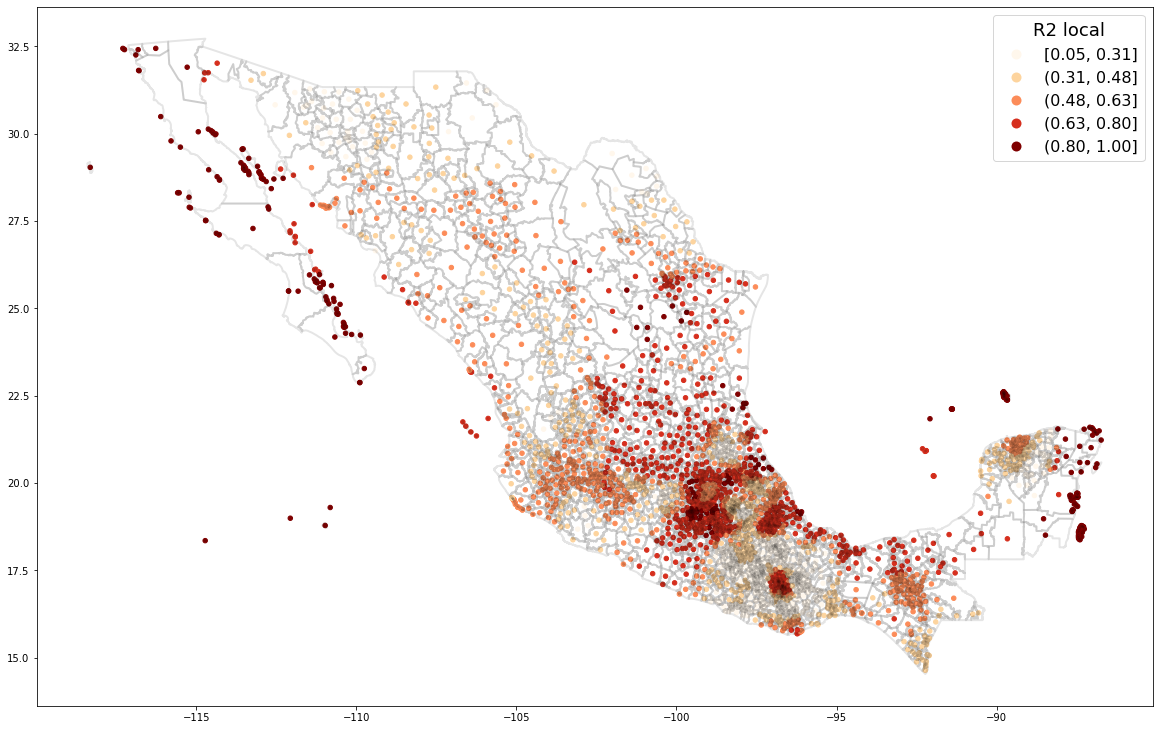
\includegraphics[scale=0.4]{output_19_1.png}
	\caption{Bondad de ajuste local usando separación Natural Breaks}
\end{figure}





%====================================================================================================
%============================================Conclucion=============================================
%====================================================================================================
\section{Conclusión}

Si bien este ensayo fue superficial, se puede ver que existen relaciones de marginalización dada por estas características de precarización en la población en diversas regiones del país. También valdría la pena analizar la relación que existe entre las zonas con altos valores de $R^2$ locales que rodea a zonas con bajas o viceversa, en vista de que estas pueden estar captando relaciones "locales" de centro-periferia en el centro y sur del país.

%====================================================================================================
%===============================================Referencias==========================================
%====================================================================================================
\begin{thebibliography}{2}

\bibitem{a} CONAPO. Cartografía de marginación por municipio 2015. CONAPO. \url{http://www.conapo.gob.mx/es/CONAPO/Datos_Abiertos_del_Indice_de_Marginacion}

\bibitem{b} Binbin Lu , Martin Charlton , Paul Harris and A. Stewart Fotheringham (2013). Geographically weighted regression with a non-Euclidean distance metric: a case study using hedonic house price data. International Journal of Geographical Information Science.

\bibitem{c}  Yuji Murayama. Progress in Geospatial Analysis. Springer.


\bibitem{d} Wikipedia. Geographical distance [online] \url{https://en.wikipedia.org/wiki/Geographical_distance}  

\end{thebibliography}


\end{document}